\section*{Numerical Verification}

Every exact formula and every limit in the preceding sections was checked by Monte Carlo simulation with fixed seeds. Table~\ref{tab:mc} reports the comparison. Each row uses \MCReps{} independent Wishart draws, except the spiked rows (400 draws at $N=400$, $n=1600$) and the dynamic row (200 Euler paths). The covariance matrices in the rows that allow a general $\Sigma$ are random, with condition numbers of 10 or 20, so the absence of $\Sigma$ from the exact formulas is itself being tested. The last column reports the proportional limit where one exists, which shows how far finite-sample values sit from their limits at the dimensions used. The exact second and third Wishart moments agree to four decimals, while the Narayana limit $1+3q+q^2$ is off by about one hundredth at $n=400$. That gap is precisely the $3(1+q)/n+4/n^2$ correction. Measured against the limit instead of the exact value, the simulated third moment would appear to deviate by more than ten standard errors, a small reminder of the theme of this paper. The log-determinant row shows that the second-order term $\tfrac12\log(1-q)$ is needed to bridge the limit $N\varphi(q)$ and the exact value. Every other exact entry lies within two Monte Carlo standard errors of its simulated counterpart. This includes the spurious information under strong dependence, its null mean and Wilks variance, both Kullback--Leibler costs, both minimum-variance ratios, the BBP outlier and overlap at two spike strengths, and the matrix Ornstein--Uhlenbeck information rate.

\begin{table}[htbp]
\centering
\caption{Monte Carlo verification of the exact and limiting formulas. ``Exact or limit'' is the analytic value used for the comparison. For the spiked rows and the dynamic row this is the large-$N$ limit or the continuous-time value. The final column gives the proportional limit where it differs. Dimensions: moments and log-determinant at $N=100$, $n=400$. Information rows at $(p,r,n)=(10,20,100)$. Kullback--Leibler rows at $N=20$, $n=100$. Portfolio rows at $N=50$, $n=200$. BBP rows at $N=400$, $n=1600$. Matrix OU at $N=10$, $a=\tfrac12$, $b=1$, Euler step $0.01$ over $20$ time units.}
\label{tab:mc}
\small
\begin{tabular}{lrrrr}
\toprule
Quantity & Exact or limit & Simulated & MC s.e. & Limit \\
\midrule
\multicolumn{5}{l}{\emph{Spectral moments and log-determinant}}\\[1pt]
\quad $N^{-1}\E\tr S^2$ (exact) & 1.2525 & 1.2521 & 0.0003 & 1.2500 \\
\quad $N^{-1}\E\tr S^3$ (exact) & 1.8219 & 1.8212 & 0.0007 & 1.8125 \\
\quad $\E\log\det S-\log\det\Sigma$ (exact) & \ensuremath{-}13.8391 & \ensuremath{-}13.8515 & 0.0119 & \ensuremath{-}13.6954 \\
\midrule
\multicolumn{5}{l}{\emph{Spurious information}}\\[1pt]
\quad $\E\hat I-I$, $(p,r,n)=(10,20,100)$ & 1.1904 & 1.1885 & 0.0037 & 1.1833 \\
\quad $\E_0\hat I$ (independence) & 1.1904 & 1.1871 & 0.0019 & -- \\
\quad $\Var_0\hat I$ (Wilks) & 0.0143 & 0.0140 & 0.0003 & 0.0141 \\
\midrule
\multicolumn{5}{l}{\emph{Information costs and portfolio risk}}\\[1pt]
\quad $\E\KL(\N_\Sigma\|\N_S)$ & 1.5283 & 1.5320 & 0.0035 & 1.4257 \\
\quad $\E\KL(\N_S\|\N_\Sigma)$ & 1.1299 & 1.1312 & 0.0018 & 1.0743 \\
\quad $\E R_{\rm in}/R$ & 0.7550 & 0.7535 & 0.0014 & 0.7500 \\
\quad $\E R_{\rm out}/R$ & 1.3267 & 1.3279 & 0.0012 & 1.3333 \\
\midrule
\multicolumn{5}{l}{\emph{Spiked covariance (BBP)}}\\[1pt]
\quad BBP outlier, $\ell=2$ & 2.5000 & 2.5043 & 0.0031 & -- \\
\quad BBP overlap$^2$, $\ell=2$ & 0.6000 & 0.5985 & 0.0022 & -- \\
\quad BBP outlier, $\ell=4$ & 4.3333 & 4.3263 & 0.0071 & -- \\
\quad BBP overlap$^2$, $\ell=4$ & 0.8974 & 0.8974 & 0.0004 & -- \\
\midrule
\multicolumn{5}{l}{\emph{Matrix Ornstein--Uhlenbeck dynamics}}\\[1pt]
\quad matrix OU KL rate & 6.8750 & 6.9439 & 0.0873 & -- \\
\bottomrule
\end{tabular}

\end{table}

The left panel of Figure~\ref{fig:spurious} plots the null mean of the plug-in information for independent blocks of equal size $p=r$ at $n=250$, with $\pm2$ standard deviation bands. The exact digamma formula and the proportional limit $n\kappa$ are indistinguishable at this scale and pass through the simulated means. The classical approximation $pr/(2n)$ is accurate for $p\leq20$ and then falls behind, reaching about $55\%$ of the true spurious information at $p=r=100$. The bands also illustrate the second message of the proportional limit. The standard deviation grows from $0.006$ at $p=2$ to only $0.54$ at $p=100$, so the spurious information becomes overwhelmingly significant as dimension grows. An uncorrected test would reject independence with probability approaching one. Table~\ref{tab:spurious} in Appendix~C reports the underlying numbers, including the exact and simulated standard deviations.

\begin{figure}[htbp]
\centering
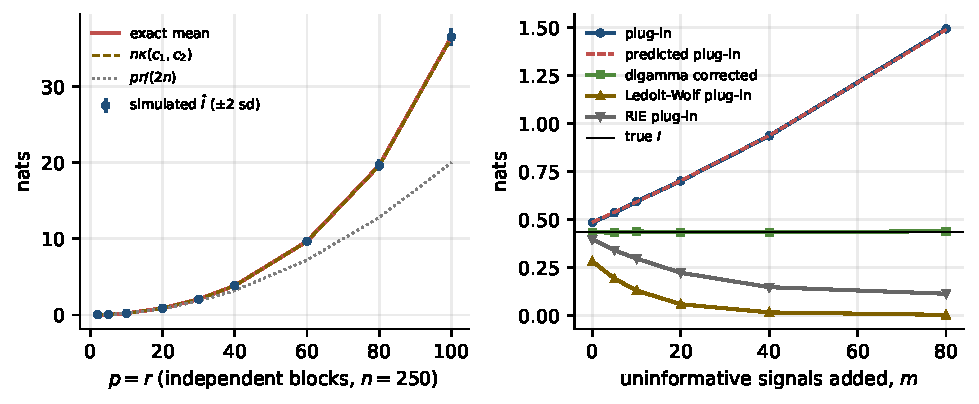
\includegraphics[width=\textwidth]{figures/spurious.pdf}
\caption{Spurious information. Left: plug-in mutual information of independent blocks with $p=r$ and $n=250$, with the exact mean $B_n(p,p)$, the proportional limit $n\kappa(p/n,p/n)$ and the classical $pr/(2n)$. Right: a design with five payoffs, five informative signals with canonical correlation $0.4$, and $m$ appended uninformative signals, at $n=250$. The plug-in estimate rises as predicted by the monotonicity proposition, the digamma-corrected estimate stays at the true value, and the Ledoit--Wolf and RIE plug-in estimates are biased towards zero.}
\label{fig:spurious}
\end{figure}

The right panel of Figure~\ref{fig:spurious} and Table~\ref{tab:noise} illustrate the monotonicity proposition and its economic reading. Five payoffs are linked to five informative signals with canonical correlations of $0.4$, so the true information is $0.436$ nats. Appending $m$ independent signals leaves the truth unchanged. The plug-in estimate nevertheless climbs from $0.485$ at $m=0$ to $1.494$ at $m=80$, matching the exact prediction $I+B_n(5,5+m)$ to within simulation error at every $m$. The digamma-corrected estimate stays between $0.433$ and $0.440$. The two cleaning estimators behave very differently. Ledoit--Wolf shrinkage removes the spurious information and much of the genuine information too, so its estimate falls to $0.004$ nats at $m=80$. The rotationally invariant estimator is less aggressive but also drifts downward, to $0.114$ nats. Shrinkage towards the identity pulls all canonical correlations towards zero, and adding noise coordinates raises the optimal shrinkage intensity. For the estimation of information, exact bias correction dominates covariance cleaning.

\begin{figure}[htbp]
\centering
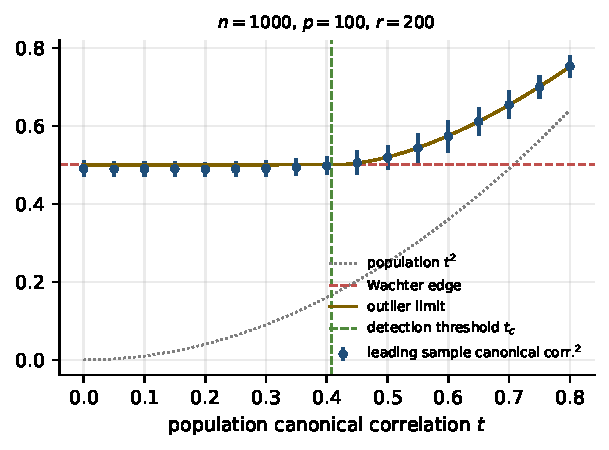
\includegraphics[width=0.68\textwidth]{figures/cca_phase.pdf}
\caption{Canonical-correlation phase transition at $n=1000$, $p=100$, $r=200$. The leading squared sample canonical correlation (mean $\pm2$ s.d. over 160 draws) sticks to the Wachter edge $\omega_+=\CCAEdge$ below the threshold $t_c=\CCAThr$ and follows the outlier limit $\gamma(t)$ of \eqref{eq:cca-spike} above it. Below the threshold, finite-$N$ draws sit slightly below $\omega_+$, as the Tracy--Widom scaling predicts.}
\label{fig:cca}
\end{figure}

Figure~\ref{fig:cca} checks the canonical-correlation transition behind the information frontier. With $c_1=0.1$ and $c_2=0.2$, the threshold is $t_c=\CCAThr$ and the Wachter edge is $\omega_+=\CCAEdge$. Below the threshold the leading squared sample canonical correlation stays at the edge, at about $0.49$ because of the negative finite-$N$ edge shift, whatever the population value. Above it, the simulated means follow $\gamma(t)$ closely. At $t=0.6$ the formula gives \CCAsixA{} and the simulation \CCAsixS{}, and at $t=0.8$ they are \CCAeightA{} and \CCAeightS{}. The information content of the threshold direction is $I_c=\FrontierSim{}$ nats. A rank-one link weaker than that is invisible to the leading canonical correlation at these dimensions, even though its value to an investor who knew its direction would be about nine percent of a unit of risk tolerance.
